% Emacs, this is -*-latex-*-

\ex{Predictive distributions for hidden Markov models}
\label{ex:predictive-distributions-for-hidden-markov-models}
For the hidden Markov model
$$ p(h_{1:d},v_{1:d}) = p(v_1|h_1)p(h_1)\prod_{i=2}^d
p(v_i|h_i)p(h_i|h_{i-1})$$ assume you have observations for $v_i$,
$i=1, \ldots, u < d$.

\begin{exenumerate}
\item \label{q:h-predictive-hmm} Use message passing to compute $p(h_t|v_{1:u})$ for $u<t\le
  d$. For the sake of concreteness, you may consider the case $d=6, u=2,
  t=4$.

  \begin{solution}
    The factor graph for $d=6, u=2$, with messages that are required
    for the computation of $p(h_t|v_{1:u})$ for $t=4$, is as follows.
    \begin{center}
      \scalebox{1}{
        \begin{tikzpicture}[ugraph,minimum size=1cm, inner sep=3pt]
          
          \node[fact, label=above:$\phi_1$] (f1) at (-1,2) {};;
          \node[cont] (h1) at (0,2) {$h_1$};
          \node[fact, label=above:$\phi_2$] (f2) at (1,2) {};
          \node[cont] (h2) at (2,2) {$h_2$};
          \node[fact, label=above: {\footnotesize$p(h_3 | h_2)$}] (f3) at (3,2) {};
          \node[cont] (h3) at (4,2) {$h_3$};
          \node[fact, label=above: {\footnotesize$p(h_4 | h_3)$}] (f4) at (5,2) {};
          \node[cont] (h4) at (6,2) {$h_4$};
          \node[fact, label=above:$p(h_5 | h_4)$] (f5) at (7,2) {};
          \node[cont] (h5) at (8,2) {$h_5$};
          \node[fact, label=above:$p(h_6 | h_5)$] (f6) at (9,2) {};
          \node[cont] (h6) at (10,2) {$h_6$};

          \node[cont] (v3) at (4,0) {$v_3$};
          \node[fact, label={[xshift=0.1cm,  yshift=0cm]left: {\footnotesize$p(v_3 | h_3)$}}] (fv3) at (4,1) {};
          \node[cont] (v4) at (6,0) {$v_4$};
          \node[fact, label={[xshift=0.1cm,  yshift=0cm]left: {\footnotesize$p(v_4 | h_4)$}}] (fv4) at (6,1) {};
          \node[cont] (v5) at (8,0) {$v_5$};
          \node[fact, label={[xshift=0.1cm,  yshift=0cm]left: {\footnotesize$p(v_5 | h_5)$}}] (fv5) at (8,1) {};
          \node[cont] (v6) at (10,0) {$v_6$};
          \node[fact, label={[xshift=0.1cm,  yshift=0cm]left: {\footnotesize$p(v_6 | h_6)$}}] (fv6) at (10,1) {};
          
          \draw(h5)--(v5);
          \draw(h6)--(v6);
          \draw(h1)--(h2);
          \draw(h2)--(h3);
          \draw(h3)--(h4);
          \draw(h4)--(h5);
          \draw(h5)--(h6);
          \draw(f1) -- (h1);    

          \draw(f1)--(h1) node[midway, above, yshift=-7pt] {$\rightarrow$};
          \draw(h1)--(f2) node[midway, above, yshift=-7pt] {$\rightarrow$};
          \draw(f2)--(h2) node[midway, above, yshift=-7pt] {$\rightarrow$};
          \draw(h2)--(f3) node[midway, above, yshift=-7pt] {$\rightarrow$};
          \draw(f3)--(h3) node[midway, above, yshift=-7pt] {$\rightarrow$};
          \draw(h3)--(f4) node[midway, above, yshift=-7pt] {$\rightarrow$};
          \draw(f4)--(h4) node[midway, above, yshift=-7pt] {\red{$\rightarrow$}};

          \draw(h4)--(f5) node[midway, above, yshift=-7pt] {\red{$\leftarrow$}};
          \draw(f5)--(h5) node[midway, above, yshift=-7pt] {$\leftarrow$};
          \draw(h5)--(f6) node[midway, above, yshift=-7pt] {$\leftarrow$};
          \draw(f6)--(h6) node[midway, above, yshift=-7pt] {$\leftarrow$};

          \draw(fv3)--(h3) node[midway, right, xshift=-7pt] {$\uparrow$};
          \draw(v3)--(fv3) node[midway, right, xshift=-7pt] {$\uparrow$};
          \draw(fv4)--(h4) node[midway, right, xshift=-7pt] {$\uparrow$};
          \draw(v4)--(fv4) node[midway, right, xshift=-7pt] {$\uparrow$};
          \draw(fv5)--(h5) node[midway, right, xshift=-7pt] {$\uparrow$};
          \draw(v5)--(fv5) node[midway, right, xshift=-7pt] {$\uparrow$};
          \draw(fv6)--(h6) node[midway, right, xshift=-7pt] {$\uparrow$};
          \draw(v6)--(fv6) node[midway, right, xshift=-7pt] {$\uparrow$};
          
        \end{tikzpicture}
      }
    \end{center}
    The messages from the unobserved visibles $v_i$ to their
    corresponding $h_i$, e.g.\ $v_3$ to $h_3$, are all one. Moreover,
    the message from the $p(h_5|h_4)$ node to $h_4$ equals one as well. This
    is because all involved factors, $p(v_i|h_i)$ and
    $p(h_i|h_{i-1})$, sum to one. Hence the factor graph reduces to a chain:
    \begin{center}
      \scalebox{1}{
        \begin{tikzpicture}[ugraph]         
          \node[fact, label=above: $\phi_1$] (f1) at (-1.5,2) {};
          \node[cont] (h1) at (0,2) {$h_1$};
          \node[fact, label=above: $\phi_2$] (f2) at (1.5,2) {};
          \node[cont] (h2) at (3,2) {$h_2$};
          \node[fact, label=above: $p(h_3|h_2)$] (f3) at (4.5,2) {};
          \node[cont] (h3) at (6,2) {$h_3$};
          \node[fact, label=above: $p(h_4|h_3)$] (f4) at (7.5,2) {};
          \node[cont] (h4) at (9,2) {$h_4$};
          \draw(f1) -- (h1)  node[midway,above,sloped] {$\rightarrow$};
          \draw(h1)--(f2);
          \draw(f2)--(h2) node[midway,above,sloped] {$\rightarrow$};
          \draw(h2)--(f3);
          \draw(f3)--(h3) node[midway,above,sloped] {$\rightarrow$};
          \draw(h3)--(f4);
          \draw(f4)--(h4) node[midway,above,sloped] {\red{$\rightarrow$}}; 
      \end{tikzpicture}}
    \end{center}
    Since the variable nodes copy the messages in case of a chain, we only show
    the factor-to-variable messages.

    The graph shows that we are essentially in the same situation as
    in filtering, with the difference that we use the factors
    $p(h_s|h_{s-1})$ for $s\ge u+1$. Hence, we can use filtering to compute
    the messages until time $s=u$ and then compute the further
    messages with the $p(h_s|h_{s-1})$ as factors. This gives the
    following algorithm:
    \begin{enumerate}
    \item Compute $\alpha(h_u)$ by filtering.
    \item For $s=u+1, \ldots, t$, compute
      \begin{equation}
        \alpha(h_s) = \sum_{h_{s-1}} p(h_s|h_{s-1}) \alpha(h_{s-1})
      \end{equation}
    \item The required predictive distribution is
      \begin{equation}
        p(h_t | v_{1:u}) = \frac{1}{Z} \alpha(h_t) \quad \quad Z = \sum_{h_t} \alpha(h_t)
      \end{equation}
    \end{enumerate}
    For $s \ge u+1$, we have that
    \begin{align}
      \sum_{h_s} \alpha(h_s) &= \sum_{h_s} \sum_{h_{s-1}} p(h_s|h_{s-1}) \alpha(h_{s-1})\\
      & =  \sum_{h_{s-1}} \alpha(h_{s-1})
    \end{align}
    since $p(h_s|h_{s-1})$ is normalised. This means that the normalising constant $Z$ above equals
    \begin{equation}
      Z = \sum_{h_u} \alpha(h_u) = p(v_{1:u})
    \end{equation}
    which is the likelihood.

    For filtering, we have seen that $\alpha(h_s) \propto
    p(h_s|v_{1:s})$, $s\le u$. The $\alpha(h_s)$ for all $s>u$ are
    proportional to $p(h_s| v_{1:u})$. This may be seen by noting that
    the above arguments hold for any $t>u$. 
  \end{solution}

\item Use message passing to compute $p(v_t|v_{1:u})$ for $u<t\le
  d$. For the sake of concreteness, you may consider the case $d=6,
  u=2, t=4$.

  \begin{solution}
    The factor graph for $d=6, u=2$, with messages that are required
    for the computation of $p(v_t|v_{1:u})$ for $t=4$, is as follows.
    \begin{center}
      \scalebox{1}{
        \begin{tikzpicture}[ugraph,minimum size=1cm, inner sep=3pt]
          
          \node[fact, label=above:$\phi_1$] (f1) at (-1,2) {};;
          \node[cont] (h1) at (0,2) {$h_1$};
          \node[fact, label=above:$\phi_2$] (f2) at (1,2) {};
          \node[cont] (h2) at (2,2) {$h_2$};
          \node[fact, label=above: {\footnotesize$p(h_3 | h_2)$}] (f3) at (3,2) {};
          \node[cont] (h3) at (4,2) {$h_3$};
          \node[fact, label=above: {\footnotesize$p(h_4 | h_3)$}] (f4) at (5,2) {};
          \node[cont] (h4) at (6,2) {$h_4$};
          \node[fact, label=above:$p(h_5 | h_4)$] (f5) at (7,2) {};
          \node[cont] (h5) at (8,2) {$h_5$};
          \node[fact, label=above:$p(h_6 | h_5)$] (f6) at (9,2) {};
          \node[cont] (h6) at (10,2) {$h_6$};

          \node[cont] (v3) at (4,0) {$v_3$};
          \node[fact, label={[xshift=0.1cm,  yshift=0cm]left: {\footnotesize$p(v_3 | h_3)$}}] (fv3) at (4,1) {};
          \node[cont] (v4) at (6,0) {$v_4$};
          \node[fact, label={[xshift=0.1cm,  yshift=0cm]left: {\footnotesize$p(v_4 | h_4)$}}] (fv4) at (6,1) {};
          \node[cont] (v5) at (8,0) {$v_5$};
          \node[fact, label={[xshift=0.1cm,  yshift=0cm]left: {\footnotesize$p(v_5 | h_5)$}}] (fv5) at (8,1) {};
          \node[cont] (v6) at (10,0) {$v_6$};
          \node[fact, label={[xshift=0.1cm,  yshift=0cm]left: {\footnotesize$p(v_6 | h_6)$}}] (fv6) at (10,1) {};
          
          \draw(h5)--(v5);
          \draw(h6)--(v6);
          \draw(h1)--(h2);
          \draw(h2)--(h3);
          \draw(h3)--(h4);
          \draw(h4)--(h5);
          \draw(h5)--(h6);
          \draw(f1) -- (h1);    

          \draw(f1)--(h1) node[midway, above, yshift=-7pt] {$\rightarrow$};
          \draw(h1)--(f2) node[midway, above, yshift=-7pt] {$\rightarrow$};
          \draw(f2)--(h2) node[midway, above, yshift=-7pt] {$\rightarrow$};
          \draw(h2)--(f3) node[midway, above, yshift=-7pt] {$\rightarrow$};
          \draw(f3)--(h3) node[midway, above, yshift=-7pt] {$\rightarrow$};
          \draw(h3)--(f4) node[midway, above, yshift=-7pt] {$\rightarrow$};
          \draw(f4)--(h4) node[midway, above, yshift=-7pt] {$\rightarrow$};

          \draw(h4)--(f5) node[midway, above, yshift=-7pt] {$\leftarrow$};
          \draw(f5)--(h5) node[midway, above, yshift=-7pt] {$\leftarrow$};
          \draw(h5)--(f6) node[midway, above, yshift=-7pt] {$\leftarrow$};
          \draw(f6)--(h6) node[midway, above, yshift=-7pt] {$\leftarrow$};

          \draw(fv3)--(h3) node[midway, right, xshift=-7pt] {$\uparrow$};
          \draw(v3)--(fv3) node[midway, right, xshift=-7pt] {$\uparrow$};
          \draw(fv4)--(h4) node[midway, right, xshift=-7pt] {$\downarrow$};
          \draw(v4)--(fv4) node[midway, right, xshift=-7pt] {\red{$\downarrow$}};
          \draw(fv5)--(h5) node[midway, right, xshift=-7pt] {$\uparrow$};
          \draw(v5)--(fv5) node[midway, right, xshift=-7pt] {$\uparrow$};
          \draw(fv6)--(h6) node[midway, right, xshift=-7pt] {$\uparrow$};
          \draw(v6)--(fv6) node[midway, right, xshift=-7pt] {$\uparrow$};
          
        \end{tikzpicture}
      }
    \end{center}
    Due to the normalised factors, as above, the messages to the right
    of $h_t$ are all one. Moreover the messages that go up from the
    $v_i$ to the $h_i, i\neq t$, are also all one. Hence the graph simplifies to a chain.
    \begin{center}
      \scalebox{1}{
        \begin{tikzpicture}[ugraph]         
          \node[fact, label=above: $\phi_1$] (f1) at (-1.5,2) {};
          \node[cont] (h1) at (0,2) {$h_1$};
          \node[fact, label=above: $\phi_2$] (f2) at (1.5,2) {};
          \node[cont] (h2) at (3,2) {$h_2$};
          \node[fact, label=above: $p(h_3|h_2)$] (f3) at (4.5,2) {};
          \node[cont] (h3) at (6,2) {$h_3$};
          \node[fact, label=above: $p(h_4|h_3)$] (f4) at (7.5,2) {};
          \node[cont] (h4) at (9,2) {$h_4$};
          \node[fact, label=above: $p(v_4|h_4)$] (fv4) at (10.5,2) {};
          \node[cont] (v4) at (12,2) {$v_4$};

          \draw(f1) -- (h1)  node[midway,above,sloped] {$\rightarrow$};
          \draw(h1)--(f2);
          \draw(f2)--(h2) node[midway,above,sloped] {$\rightarrow$};
          \draw(h2)--(f3);
          \draw(f3)--(h3) node[midway,above,sloped] {$\rightarrow$};
          \draw(h3)--(f4);
          \draw(f4)--(h4) node[midway,above,sloped] {\blue{$\rightarrow$}};
          \draw(h4)--(fv4);
          \draw(fv4)--(v4) node[midway,above,sloped] {\red{$\rightarrow$}};
      \end{tikzpicture}}
    \end{center}
    The message in blue is proportional to $p(h_t|v_{1:u})$ computed
    in question \ref{q:h-predictive-hmm}. Thus assume that we have
    computed $p(h_t|v_{1:u})$. The predictive distribution on the
    level of the visibles thus is
    \begin{equation}
      p(v_t | v_{1:u}) = \sum_{h_t} p(v_t|h_t) p(h_t|v_{1:u}).
    \end{equation}
    This follows from message passing since the last node ($h_4$ in
    the graph) just copies the (normalised) message and the next
    factor equals $p(v_t|h_t)$.

    An alternative derivation follows from basic definitions and
    operations, together with the independencies in HMMs:
    \begin{align}
    &\text{\scriptsize (sum rule)}&  p(v_t | v_{1:u}) &= \sum_{h_t} p(v_t, h_t|v_{1:u})\\
    &\text{\scriptsize (product rule)}&  & = \sum_{h_t} p(v_t|h_t, v_{1:u}) p(h_t|v_{1:u})\\
    &\text{\scriptsize ($v_t \independent v_{1:u} \mid h_t$)}&  & = \sum_{h_t} p(v_t|h_t) p(h_t|v_{1:u})
    \end{align}
  \end{solution}
  
\end{exenumerate}
% ---------------------------------------

\ex{Viterbi algorithm}

For the hidden Markov model
$$ p(h_{1:t},v_{1:t}) = p(v_1|h_1)p(h_1)\prod_{i=2}^t
p(v_i|h_i)p(h_i|h_{i-1})$$ assume you have observations for $v_i$,
$i=1, \ldots, t$. Use the max-sum algorithm to derive an iterative algorithm to compute
\begin{equation}
  \hat{\h} = \argmax_{h_1, \ldots, h_t}  p(h_{1:t}|v_{1:t})
\end{equation}
Assume that the latent variables $h_i$ can take $K$ different values,
e.g.\ $h_i \in \{0,\ldots, K-1\}$. The resulting algorithm is known as
Viterbi algorithm.

\begin{solution}
  
  We first form the factors
  \begin{align}
    \phi_1(h_1) &= p(v_1|h_1) p(h_1)& \phi_2(h_1, h_2) &= p(v_2|h_2) p(h_2|h_1)\\
    \ldots      &                  & \phi_t(h_{t-1},h_t) &= p(v_t|h_t) p(h_{t}|h_{t-1})
  \end{align}
 where the $v_i$ are known and fixed. The posterior $p(h_1, \ldots,
 h_t | v_1, \ldots, v_t)$ is then represented by the following factor
 graph (assuming $t=4$).
  
  \begin{center}
    \scalebox{1}{
      \begin{tikzpicture}[ugraph]         
        \node[fact, label=above: $\phi_1$] (f1) at (-1.5,2) {};
        \node[cont] (h1) at (0,2) {$h_1$};
        \node[fact, label=above: $\phi_2$] (f2) at (1.5,2) {};
        \node[cont] (h2) at (3,2) {$h_2$};
        \node[fact, label=above: $\phi_3$] (f3) at (4.5,2) {};
        \node[cont] (h3) at (6,2) {$h_3$};
        \node[fact, label=above: $\phi_4$] (f4) at (7.5,2) {};
        \node[cont] (h4) at (9,2) {$h_4$};
        
        \draw(f1)--(h1);
        \draw(h1)--(f2);
        \draw(f2)--(h2);
        \draw(h2)--(f3);
        \draw(f3)--(h3);
        \draw(h3)--(f4);
        \draw(f4)--(h4);
    \end{tikzpicture}}
  \end{center}

  For the max-sum algorithm, we here choose $h_t$ to be the root. We
  thus initialise the algorithm with $\mfxmess{\phi_1}{h_1}{1}(h_1) =
  \log \phi_1(h_1) = \log p(v_1|h_1) + \log p(h_1)$ and then compute the
  messages from left to right, moving from the leaf $\phi_1$ to the
  root $h_t$.

  Since we are dealing with a chain, the variable nodes, much like in
  the sum-product algorithm, just copy the incoming messages. It thus
  suffices to compute the factor to variable messages shown in the
  graph, and then backtrack to $h_1$.
  
 \begin{center}
      \scalebox{1}{
        \begin{tikzpicture}[ugraph]         
          \node[fact, label=above: $\phi_1$] (f1) at (-1.5,2) {};
          \node[cont] (h1) at (0,2) {$h_1$};
          \node[fact, label=above: $\phi_2$] (f2) at (1.5,2) {};
          \node[cont] (h2) at (3,2) {$h_2$};
          \node[fact, label=above: $\phi_3$] (f3) at (4.5,2) {};
          \node[cont] (h3) at (6,2) {$h_3$};
          \node[fact, label=above: $\phi_4$] (f4) at (7.5,2) {};
          \node[cont] (h4) at (9,2) {$h_4$};

          \draw(f1) -- (h1)  node[midway,above,sloped] {$\rightarrow$};
          \draw(h1)--(f2);
          \draw(f2)--(h2) node[midway,above,sloped] {$\rightarrow$};
          \draw(h2)--(f3);
          \draw(f3)--(h3) node[midway,above,sloped] {$\rightarrow$};
          \draw(h3)--(f4);
          \draw(f4)--(h4) node[midway,above,sloped] {$\rightarrow$};
      \end{tikzpicture}}
 \end{center}

 With $\mxfmess{h_{i-1}}{\phi_i}{1}(h_{i-1})=\mfxmess{\phi_{i-1}}{h_{i-1}}{1}(h_{i-1})$, the factor-to-variable update equation is
 \begin{align}
   \mfxmess{\phi_i}{h_i}{1}(h_i) &= \max_{h_{i-1}} \log \phi_i(h_{i-1}, h_i) + \mxfmess{h_{i-1}}{\phi_i}{1}(h_{i-1})\\
   &= \max_{h_{i-1}} \log \phi_i(h_{i-1}, h_i) + \mfxmess{\phi_{i-1}}{h_{i-1}}{1}(h_{i-1})
 \end{align}
 To simplify notation, denote $\mfxmess{\phi_i}{h_i}{1}(h_i)$ by $V_i(h_i)$. We thus have
 \begin{align}
   V_1(h_1) & = \log p(v_1|h_1) + \log p(h_1) \\
   V_i(h_i) & =  \max_{h_{i-1}} \log \phi_i(h_{i-1}, h_i) + V_{i-1}(h_{i-1}) \quad \quad i=2, \ldots, t
 \end{align}
 In general, $V_1(h_1)$ and $V_i(h_i)$ are functions that depend on
 $h_1$ and $h_i$, respectively.  Assuming that the $h_i$ can take on
 the values $0, \ldots, K-1$, the above equations can be written as
\begin{align}
  v_{1,k} &= \log p(v_1|k) + \log p(k) &  k&=0, \ldots, K-1\\
  v_{i,k} & =  \max_{m \in{0, \ldots, K-1}} \log \phi_i(m, k) + v_{i-1,m} &  k&=0, \ldots, K-1, \quad i=2, \ldots, t,
 \end{align}
At the end of the algorithm, we thus have a $t \times K$ matrix $\V$
with elements $v_{i,k}$.

The maximisation can be performed by computing the temporary matrix
$\A$ (via broadcasting) where the $(m,k)$-th element is $\log
\phi_i(m, k) + v_{i-1,m}$. Maximisation then corresponds to
determining the maximal value in each column.

To support the backtracking, when we compute $V_i(h_i)$ by maximising
over $h_{i-1}$, we compute at the same time the look-up table
\begin{equation}
  \gamma_i^*(h_i)   =  \argmax_{h_{i-1}} \log \phi_i(h_{i-1}, h_i) + V_{i-1}(h_{i-1})
\end{equation}
When $h_i$ takes on the values $0, \ldots, K-1$, this can be written as
\begin{equation}
  \gamma^*_{i,k} = \argmax_{m \in{0, \ldots, K-1}} \log \phi_i(m, k) + v_{i-1,m}
\end{equation}
This is the (row) index of the maximal element in each column of the temporary matrix $\A$.

After computing $v_{t,k}$ and $\gamma^*_{t,k}$, we then perform
backtracking via
\begin{align}
  \hat{h}_t & = \argmax_{k}   v_{t,k}\\
  \hat{h}_i & = \gamma^*_{i+1,\hat{h}_{i+1}} \quad \quad i=t-1, \ldots, 1
\end{align}
This gives recursively $\hat{\h} = (\hat{h}_1, \ldots, \hat{h}_t) = \argmax_{h_1, \ldots, h_t}  p(h_{1:t}|v_{1:t})$.

\end{solution}

% ---------------------------------------

\ex{Forward filtering backward sampling for hidden Markov models}
\label{ex:FFBS}

Consider the hidden Markov model specified by the following DAG.

\begin{center}
  \scalebox{0.8}{
    \begin{tikzpicture}[dgraph, minimum size=0.5cm, inner sep=3pt]
      \node[cont] (h1) at (0,2) {$h_1$};
      \node       (aa) at (1,2) {};
      \node       (bb) at (2,2) {$\ldots$};
      \node       (cc) at (2,0) {$\ldots$};
      \node       (dd) at (3,2) {};

      \node[cont, inner sep=0em] (h2) at (5,2) {$h_{t-1}$};
      \node[cont] (h3) at (7,2) {$h_{t}$};
      
      \node       (a) at (8,2) {};
      \node       (b) at (9,2) {$\ldots$};
      \node       (c) at (9,0) {$\ldots$};
      \node       (d) at (10,2) {};
      
      \node[cont] (h4) at (12,2) {$h_n$};

      \node[cont] (v1) at (0,0) {$v_1$};
      \node[cont, inner sep=0em] (v2) at (5,0) {$v_{t-1}$};
      \node[cont] (v3) at (7,0) {$v_t$};
      \node[cont] (v4) at (12,0) {$v_n$};
      \draw(h1)--(v1);\draw(h2)--(v2);\draw(h3)--(v3);\draw(h4)--(v4);
      \draw(h1)--(aa);\draw(dd)--(h2);\draw(h2)--(h3);\draw(h3)--(a);\draw(d)--(h4);
  \end{tikzpicture}}
\end{center}
We assume that have already run the alpha-recursion (filtering) and
can compute $p(h_t | v_{1:t})$ for all $t$. The goal is now to
generate samples $p(h_1, \ldots, h_n | v_{1:n})$, i.e.\ entire
trajectories $(h_1, \ldots, h_n)$ from the posterior. Note that this is
not the same as sampling from the $n$ filtering distributions $p(h_t |
v_{1:t})$. Moreover, compared to the Viterbi algorithm, the sampling approach
generates samples from the full posterior rather than just returning
the most probable state and its corresponding probability.

\begin{exenumerate}
\item Show that $p(h_1, \ldots, h_n|v_{1:n})$ forms a
  first-order Markov chain.

  \begin{solution}
    There are several ways to show this. The simplest is to notice
    that the undirected graph for the hidden Markov model is the same
    as the DAG but with the arrows removed as there are no colliders
    in the DAG. Moreover, conditioning corresponds to removing nodes
    from an undirected graph. This leaves us with a chain that
    connects the $h_i$.
    \begin{center}
      \scalebox{0.8}{
        \begin{tikzpicture}[ugraph]
          \node[cont] (h1) at (0,2) {$h_1$};
          \node[cont] (h2) at (2,2) {$h_2$};
          \node[cont] (h3) at (4,2) {$h_3$};
          \node       (a) at (6,2) {};
          \node       (b) at (7,2) {$\ldots$};
          \node       (d) at (8,2) {};
          \node[cont] (h4) at (10,2) {$h_n$};
          \draw(h1)--(h2);\draw(h2)--(h3);\draw(h3)--(a);\draw(d)--(h4);
      \end{tikzpicture}}
    \end{center}
    
  By graph separation, we see that $p(h_1,\ldots, h_n|v_{1:n})$ forms
  a first-order Markov chain so that e.g.\ $h_{1:t-1} \independent
  h_{t+1:n} | h_t$ (past independent from the future given the
  present).
    
  \end{solution}
  
  \item Since $p(h_1, \ldots, h_n|v_{1:n})$ is a first-order Markov
    chain, it suffices to determine $p(h_{t-1}|h_t, v_{1:n})$, the
    probability mass function for $h_{t-1}$ given $h_t$ and
    all the data $v_{1:n}$. Use message passing to show
    that
    \begin{equation}
      p(h_{t-1}, h_t| v_{1:n}) \propto \alpha(h_{t-1}) \beta(h_t) p(h_t|h_{t-1})p(v_t|h_t) 
    \end{equation}

    \begin{solution}
      Since all visibles are in the conditioning set, i.e.\ assumed
      observed, we can represent the conditional model $p(h_1, \ldots,
      h_n|v_{1:n})$ as a chain factor tree, e.g.\ as follows in case
      of $n=4$
      \begin{center}
        \scalebox{1}{
          \begin{tikzpicture}[ugraph]         
            \node[fact, label=above: $\phi_1$] (f1) at (-1.5,2) {};
            \node[cont] (h1) at (0,2) {$h_1$};
            \node[fact, label=above: $\phi_2$] (f2) at (1.5,2) {};
            \node[cont] (h2) at (3,2) {$h_2$};
            \node[fact, label=above: $\phi_3$] (f3) at (4.5,2) {};
            \node[cont] (h3) at (6,2) {$h_3$};
            \node[fact, label=above: $\phi_4$] (f4) at (7.5,2) {};
            \node[cont] (h4) at (9,2) {$h_4$};
            \draw(f1) -- (h1);
            \draw(h1)--(f2);
            \draw(f2)--(h2);
            \draw(h2)--(f3);
            \draw(f3)--(h3);
            \draw(h3)--(f4);
            \draw(f4)--(h4);
        \end{tikzpicture}}
      \end{center}
      Combining the emission distributions $p(v_s|h_s)$ (and marginal
      $p(h_1)$) with the transition distributions $p(h_s|h_{s-1})$ we
      obtain the factors
       \begin{align}
         \phi_1(h_1) & = p(h_1) p(v_1|h_1)\\
         \phi_s(h_{s-1}, h_s) &= p(h_s|h_{s-1})p(v_s|h_s) \quad \text{for } t=2, \ldots, n
       \end{align}
       We see from the factor tree that $h_{t-1}$ and $h_t$ are
       neighbours, being attached to the same factor node
       $\phi_t(h_{t-1}, h_t)$, e.g. $\phi_3$ in case of $p(h_{2}, h_3 | v_{1:4})$.

       By the rules of message passing, the joint $p(h_{t-1}, h_{t} |
       v_{1:n})$ is thus proportional to $\phi_t$ times the messages
       into $\phi_t$. The following graph shows the messages for the
       case of $p(h_{2}, h_3 | v_{1:4})$.
       \begin{center}
         \scalebox{1}{
           \begin{tikzpicture}[ugraph]         
             \node[fact, label=above: $\phi_1$] (f1) at (-1.5,2) {};
             \node[cont] (h1) at (0,2) {$h_1$};
             \node[fact, label=above: $\phi_2$] (f2) at (1.5,2) {};
             \node[cont] (h2) at (3,2) {$h_2$};
             \node[fact, label=above: $\phi_3$] (f3) at (4.5,2) {};
             \node[cont] (h3) at (6,2) {$h_3$};
             \node[fact, label=above: $\phi_4$] (f4) at (7.5,2) {};
             \node[cont] (h4) at (9,2) {$h_4$};
             \draw(f1) -- (h1);
             \draw(h1)--(f2);
             \draw(f2)--(h2);
             \draw(h2)--(f3) node[midway,above,sloped] {$\rightarrow$};
             \draw(f3)--(h3) node[midway,above,sloped] {$\leftarrow$}; 
             \draw(h3)--(f4);
             \draw(f4)--(h4);
         \end{tikzpicture}}
       \end{center}
       Since the variable nodes only receive single messages from any
       direction, they copy the messages so that the messages into
       $\phi_t$ are given by $\alpha(h_{t-1})$ and $\beta(h_t)$ shown
       below in red and blue, respectively.
       \begin{center}
         \scalebox{1}{
           \begin{tikzpicture}[ugraph]         
             \node[fact, label=above: $\phi_1$] (f1) at (-1.5,2) {};
             \node[cont] (h1) at (0,2) {$h_1$};
             \node[fact, label=above: $\phi_2$] (f2) at (1.5,2) {};
             \node[cont] (h2) at (3,2) {$h_2$};
             \node[fact, label=above: $\phi_3$] (f3) at (4.5,2) {};
             \node[cont] (h3) at (6,2) {$h_3$};
             \node[fact, label=above: $\phi_4$] (f4) at (7.5,2) {};
             \node[cont] (h4) at (9,2) {$h_4$};
             \draw(f1) -- (h1);
             \draw(h1)--(f2);
             \draw(f2)--(h2) node[midway,above,sloped] {\red{$\rightarrow$}};
             \draw(h2)--(f3);
             \draw(f3)--(h3);
             \draw(h3)--(f4) node[midway,above,sloped] {\blue{$\leftarrow$}}; 
             \draw(f4)--(h4);
         \end{tikzpicture}}
       \end{center}
       Hence, 
       \begin{align}
         p(h_{t-1}, h_t| v_{1:n}) &\propto \alpha(h_{t-1}) \beta(h_t) \phi_t(h_{t-1}, h_t)\\
         &\propto \alpha(h_{t-1}) \beta(h_t) p(h_t|h_{t-1}) p(v_t|h_t)
       \end{align}
       which is the result that we want to show.
    \end{solution}


  \item Show that $p(h_{t-1}|h_t, v_{1:n}) = \frac{\alpha(h_{t-1})}{\alpha(h_t)} p(h_t|h_{t-1}) p(v_t|h_t)$.
   
    \begin{solution}
      The conditional $p(h_{t-1}|h_t, v_{1:n})$ can be written as the ratio
      \begin{equation}
        p(h_{t-1}|h_t, v_{1:n}) = \frac{p(h_{t-1}, h_t| v_{1:n})}{p(h_t|v_{1:n})}.
      \end{equation}
      Above, we have shown that the numerator satisfies
      \begin{equation}
        p(h_{t-1}, h_t| v_{1:n}) \propto \alpha(h_{t-1}) \beta(h_t) p(h_t|h_{t-1}) p(v_t|h_t).
      \end{equation}
      The denominator $p(h_t|v_{1:n})$ is proportional to $\alpha(h_t)
      \beta(h_t)$ since it is the smoothing distribution than can be
      determined via the alpha-beta recursion.

      Normally, we needed to sum the messages over all values of
      $(h_{t-1},h_t)$ to find the normalising constant of the
      numerator. For the denominator, we had to sum over all values of
      $h_t$. Next, I will argue qualitatively that this summation is
      not needed; the normalising constants are both equal to
      $p(v_{1:t})$. A more mathematical argument is given below.

      We started with a factor graph and factors that represent the
      joint $p(h_{1:n}, v_{1:n})$. The conditional $p(h_{1:n},
      v_{1:n})$ equals
      \begin{equation}
        \label{eq:h-given-v-hmm}
        p(h_{1:n} | v_{1:n}) = \frac{p(h_{1:n}, v_{1:n})}{p(v_{1:n})}
      \end{equation}
      Message passing is variable elimination. Hence, when computing
      $p(h_t|v_{1:n})$ as $\alpha(h_t) \beta(h_t)$ from a factor graph
      for $p(h_{1:n}, v_{1:n})$, we only need to divide by
      $p(v_{1:n})$ for normalisation; explicitly summing out $h_t$ is
      not needed. In other words,
      \begin{equation}
        p(h_t|v_{1:n}) =  \frac{\alpha(h_t) \beta(h_t)}{p(v_{1:n})}.
      \end{equation}
      Similarly, $p(h_{t-1}, h_t|v_{1:n})$ is also obtained from
      \eqref{eq:h-given-v-hmm} by marginalisation/variable
      elimination. Again, when computing $p(h_{t-1}, h_t|v_{1:n})$ as
      $\alpha(h_{t-1}) \beta(h_t) p(h_t|h_{t-1}) p(v_t|h_t)$ from a
      factor graph for $p(h_{1:n}, v_{1:n})$, we do not need to
      explicitly sum over all values of $h_t$ and $h_{t-1}$ for
      normalisation. The definition of the factors in the factor graph
      together with \eqref{eq:h-given-v-hmm} shows that we can simply
      divide by $p(v_{1:n})$. This gives
      \begin{align}
        p(h_{t-1}, h_t| v_{1:n}) & = \frac{1}{p(v_{1:n})} \alpha(h_{t-1}) \beta(h_t) p(h_t|h_{t-1}) p(v_t|h_t).
      \end{align}

      The desired conditional thus is
      \begin{align}
        p(h_{t-1} | h_t, v_{1:n}) & = \frac{p(h_{t-1}, h_t| v_{1:n})}{p(h_t|v_{1:n})} \\
        & = \frac{\alpha(h_{t-1}) \beta(h_t) p(h_t|h_{t-1}) p(v_t|h_t)}{\alpha(h_t) \beta(h_t)}\\
        & = \frac{\alpha(h_{t-1}) p(h_t|h_{t-1}) p(v_t|h_t)}{\alpha(h_t)}
      \end{align}
      which is the result that we wanted to show. Note that
      $\beta(h_t)$ cancels out and that $p(h_{t-1} | h_t, v_{1:n})$
      only involves the $\alpha$'s, the (forward) transition
      distribution $p(h_t|h_{t-1})$ and the emission distribution at
      time $t$.

      \emph{Alternative solution:} An alternative, mathematically rigorous
      solution is as follows.  The conditional $p(h_{t-1}|h_t,
      v_{1:n})$ can be written as the ratio
      \begin{equation}
        p(h_{t-1}|h_t, v_{1:n}) = \frac{p(h_{t-1}, h_t| v_{1:n})}{p(h_t|v_{1:n})}.
      \end{equation}
      We first determine the denominator. From the properties of the
      alpha and beta recursion, we know that
      \begin{align}
        \alpha(h_{t}) &= p(h_{t}, v_{1:t}) & \beta(h_t) = p(v_{t+1:n}|h_t)
      \end{align}
      Using that $v_{t+1:n} \independent v_{1:t} | h_t$, we can thus
      express the denominator $p(h_t|v_{1:n})$ as
      \begin{align}
        p(h_t|v_{1:n}) &= \frac{p(h_t, v_{1:n})}{p(v_{1:n})}\\
        & = \frac{p(h_t, v_{1:t}) p(v_{t+1:n}|h_t)}{p(v_{1:n})}\\
        & = \frac{\alpha(h_t) \beta(h_t)}{p(v_{1:n})}
      \end{align}
      
      For the numerator, we have
      \begin{align}
        p(h_{t-1},h_t | v_{1:n}) & =  \frac{p(h_{t-1},h_t, v_{1:n})}{p(v_{1:n})} \\
        & = \frac{p(h_{t-1}, v_{1:t-1}, h_t, v_{t:n})}{p(v_{1:n})} \\
        & = \frac{p(h_{t-1}, v_{1:t-1}) p(h_t, v_{t:n} | h_{t-1}, v_{1:t-1})}{p(v_{1:n})} \\
        & = \frac{p(h_{t-1}, v_{1:t-1}) p(h_t, v_{t:n} | h_{t-1})}{p(v_{1:n})} \quad \quad \text{\small (using $h_t, v_{1:t} \independent v_{1:t-1} | h_{t-1}$)}\\
        & = \frac{\alpha(h_{t-1}) p(h_t, v_{t:n} | h_{t-1})}{p(v_{1:n})} \quad \quad \text{\small (using $\alpha(h_{t-1}) = p(h_{t-1}, v_{1:t-1})$)}
      \end{align}
      With the product rule, we have  $p(h_t, v_{t:n} | h_{t-1}) =  p(v_t|h_t, h_{t-1}, v_{t+1:n}) p(h_t, v_{t+1:n} | h_{t-1})$ so that
      \begin{align}   
  p(h_{t-1},h_t | v_{1:n})& = \frac{\alpha(h_{t-1}) p(v_t|h_t, h_{t-1}, v_{t+1:n}) p(h_t, v_{t+1:n} | h_{t-1})}{p(v_{1:n})}\\
       & = \frac{\alpha(h_{t-1}) p(v_t|h_t) p(h_t, v_{t+1:n} | h_{t-1})}{p(v_{1:n})} \quad \quad \text{\small (using $v_t \independent h_{t-1}, v_{t+1:n} |h_t$)}\\
        & = \frac{\alpha(h_{t-1}) p(v_t|h_t) p(h_t | h_{t-1}) p(v_{t+1:n} | h_{t-1}, h_t)}{p(v_{1:n})} 
        \end{align}
        Hence
        \begin{align}
       p(h_{t-1},h_t | v_{1:n}) & = \frac{\alpha(h_{t-1}) p(v_t|h_t) p(h_t | h_{t-1}) p(v_{t+1:n} | h_t)}{p(v_{1:n})} \quad \quad \text{\small (using $v_{t+1:n} \independent h_{t-1} | h_t$)}\\
& = \frac{\alpha(h_{t-1}) p(v_t|h_t) p(h_t | h_{t-1}) \beta(h_t)}{p(v_{1:n})} \quad \quad \text{\small (using $\beta(h_t) = p(v_{t+1:n}|h_t)$)}
      \end{align}

      The desired conditional thus is
      \begin{align}
        p(h_{t-1} | h_t, v_{1:n}) & = \frac{p(h_{t-1}, h_t| v_{1:n})}{p(h_t|v_{1:n})} \\
        & = \frac{\alpha(h_{t-1}) \beta(h_t) p(h_t|h_{t-1}) p(v_t|h_t)}{\alpha(h_t) \beta(h_t)}\\
        & = \frac{\alpha(h_{t-1}) p(h_t|h_{t-1}) p(v_t|h_t)}{\alpha(h_t)}
      \end{align}
      which is the result that we wanted to show.
    \end{solution}

    We thus obtain the following algorithm to generate samples from
    $p(h_1, \ldots, h_n|v_{1:n})$:
    \begin{enumerate}
    \item Run the alpha-recursion (filtering) to determine all
      $\alpha(h_t)$ forward in time for $t=1, \ldots, n$.
    \item Sample $h_n$ from $p(h_n | v_{1:n}) \propto \alpha(h_n)$
    \item Go backwards in time using
      \begin{equation}
        p(h_{t-1}|h_t, v_{1:n}) = \frac{\alpha(h_{t-1})}{\alpha(h_t)} p(h_t|h_{t-1}) p(v_t|h_t)
      \end{equation}
      to generate samples $h_{t-1}|h_t, v_{1:n}$ for $t=n, \ldots, 2$.
    \end{enumerate}
    This algorithm is known as forward filtering backward sampling (FFBS). 
    
\end{exenumerate}


% ----------------------------------------

 \ex{Prediction exercise}
 
 Consider a hidden Markov model with three visibles $v_1, v_2, v_3$
 and three hidden variables $h_1, h_2, h_3$ which can be represented
 with the following factor graph:
 
 \begin{center}
   \scalebox{0.9}{
     \begin{tikzpicture}[ugraph,minimum size=1cm, inner sep=3pt]
       \node[cont] (v1) at (0,0) {$v_1$};
       \node[fact, label={[xshift=0.1cm,  yshift=0cm]left: $p(v_1 | h_1)$}] (fv1) at (0,1) {};
       \node[cont] (v2) at (3,0) {$v_2$};
       \node[fact, label={[xshift=0.1cm,  yshift=0cm]left: $p(v_2 | h_2)$}] (fv2) at (3,1) {};
       \node[cont] (v3) at (6,0) {$v_3$};
       \node[fact, label={[xshift=0.1cm,  yshift=0cm]left: $p(v_3 | h_3)$}] (fv3) at (6,1) {};
       
       \node[fact, label=left: $p(h_1)$] (f1) at (-1.5,2) {};
       \node[cont] (h1) at (0,2) {$h_1$};
       \node[fact, label={[label distance=-7pt]above: $p(h_2 | h_1)$}] (f2) at (1.5,2) {};
       \node[cont] (h2) at (3,2) {$h_2$};
       \node[fact, label={[label distance=-7pt]above: $p(h_3 | h_2)$}] (f3) at (4.5,2) {};
       \node[cont] (h3) at (6,2) {$h_3$};

       \draw(h1)--(v1);
       \draw(h2)--(v2);
       \draw(h3)--(v3);
       \draw(h1)--(h2);
       \draw(h2)--(h3);
       \draw(f1) -- (h1);
       
   \end{tikzpicture}}
 \end{center}
 This question is about computing the predictive probability $p(v_3=1 | v_1 =1)$.

\begin{exenumerate}
  
\item The factor graph below represents $p(h_1, h_2, h_3, v_2, v_3
  \mid v_1 =1)$. Provide an equation that defines $\phi_A$ in terms of
  the factors in the factor graph above. 

  \begin{center}
    \scalebox{0.9}{
      \begin{tikzpicture}[ugraph,minimum size=1cm, inner sep=3pt]
        \node[cont] (v2) at (3,0) {$v_2$};
        \node[fact, label={[xshift=0.1cm,  yshift=0cm]left: $p(v_2 | h_2)$}] (fv2) at (3,1) {};
        \node[cont] (v3) at (6,0) {$v_3$};
        \node[fact, label={[xshift=0.1cm,  yshift=0cm]left: $p(v_3 | h_3)$}] (fv3) at (6,1) {};
        
        \node[cont] (h1) at (0,2) {$h_1$};
        \node[fact, label={[label distance=-7pt]above: $\phi_A$}] (f2) at (1.5,2) {};
        \node[cont] (h2) at (3,2) {$h_2$};
        \node[fact, label={[label distance=-7pt]above: $p(h_3 | h_2)$}] (f3) at (4.5,2) {};
        \node[cont] (h3) at (6,2) {$h_3$};
        
        \draw(h2)--(v2);
        \draw(h3)--(v3);
        \draw(h1)--(h2);
        \draw(h2)--(h3);
                
    \end{tikzpicture}}
  \end{center}

  \begin{solution}
    
    $\phi_A(h_1, h_2) \propto p(v_1 | h_1) p(h_1) p(h_2 | h_1)$ with $v_1=1$.
    
  \end{solution}
  
\item Assume further that all variables are
  binary, $h_i \in \{0,1\}$, $v_i \in \{0,1\}$; that $p(h_1=1)=0.5$, and that the transition and emission distributions are, for all $i$, given by:

  \begin{center}
    \begin{tabular}{lll}
      \toprule
      $p(h_{i+1}|h_i)$ & $h_{i+1}$ &$h_i$ \\
      \midrule
      0 & 0 & 0\\
      1 & 1 & 0\\
      1 & 0 & 1\\
      0 & 1 & 1\\
      \bottomrule
    \end{tabular}
    \hspace{5ex}
    \begin{tabular}{lll}
      \toprule
      $p(v_i|h_i)$ & $v_i$ &$h_i$ \\
      \midrule
      0.6 & 0 & 0\\
      0.4 & 1 & 0\\
      0.4 & 0 & 1\\
      0.6 & 1 & 1\\
      \bottomrule
    \end{tabular}
  \end{center}
  Compute the numerical values of the factor $\phi_A$.

  \begin{solution}


  \item Given the definition of the transition and emission
    probabilities, we have $\phi_A(h_1,h_2) = 0$ if $h_1=h_2$. For $h_1=0, h_2 =1$, we obtain
    \begin{align}
      \phi_A(h_1=0, h_2=1) &= p(v_1=1 | h_1=0) p(h_1=0) p(h_2=1 | h_1=0) \\
      & = 0.4 \cdot 0.5 \cdot 1\\
      & = \frac{4}{10} \cdot \frac{1}{2}\\
      & = \frac{2}{10} = 0.2
    \end{align}
    For $h_1=1, h_2 =0$, we obtain
    \begin{align}
      \phi_A(h_1=1, h_2=0) &= p(v_1=1 | h_1=1) p(h_1=1) p(h_2=0 | h_1=1) \\
      & = 0.6 \cdot 0.5 \cdot 1\\
      & = \frac{6}{10} \cdot \frac{1}{2}\\
      & = \frac{3}{10} =0.3
    \end{align}
    Hence
     \begin{center}
     \begin{tabular}{lll}
      \toprule
   $\phi_A(h_1, h_2)$ & $h_1$ &$h_2$ \\
      \midrule
      0 & 0 & 0\\
      0.3 & 1 & 0\\
      0.2 & 0 & 1\\
      0 & 1 & 1\\
      \bottomrule
    \end{tabular}
  \end{center}
    
  \end{solution}

\item  Denote the message from variable node $h_2$ to factor node $p(h_3 |
  h_2)$ by $\alpha(h_2)$. Use message passing to compute $\alpha(h_2)$
  for $h_2=0$ and $h_2=1$. Report the values of any intermediate
  messages that need to be computed for the computation of
  $\alpha(h_2)$.

  \begin{solution}
    
    The message from $h_1$ to $\phi_A$ is one. The message from
    $\phi_A$ to $h_2$ is 
    \begin{align}
      \fxmess{\phi_A}{h_2}{1}(h_2=0) & = \sum_{h_1} \phi_A(h_1, h_2=0)\\
      & = 0.3\\
      \fxmess{\phi_A}{h_2}{1}(h_2=1) & = \sum_{h_1} \phi_A(h_1, h_2=1)\\
      & = 0.2
    \end{align}
    
    Since $v_2$ is not observed and $p(v_2|h_2)$ normalised, the message from $p(v_2|h_2)$ to $h_2$ equals one.

    This means that the message from $h_2$ to $p(h_3 | h_2)$, which is
    $\alpha(h_2)$ equals $\fxmess{\phi_A}{h_2}{1}(h_2)$, i.e.\ 
    \begin{align}
      \alpha(h_2=0) & = 0.3\\
      \alpha(h_2=1) & = 0.2
    \end{align}

  \end{solution}
  
\item With $\alpha(h_2)$ defined as above, use message passing to show
  that the predictive probability $p(v_3=1 | v_1=1)$ can be expressed in terms of $\alpha(h_2)$
  as
  \begin{equation}
    p(v_3=1 | v_1=1) = \frac{ x \alpha(h_2=1) + y \alpha(h_2=0)}{\alpha(h_2=1)+\alpha(h_2=0)}
  \end{equation}
  and report the values of $x$ and $y$.  

  \begin{solution}

    
    Given the definition of $p(h_3| h_2)$, the message $\fxmess{p(h_3|h_2)}{h_3}{1}(h_3)$ is
    \begin{align}
      \fxmess{p(h_3|h_2)}{h_3}{1}(h_3=0) & = \alpha(h_2 =1)\\
      \fxmess{p(h_3|h_2)}{h_3}{1}(h_3=1) & = \alpha(h_2 =0)
  \end{align}
    
  The variable node $h_3$ copies the message so that we have
  \begin{align}
    \fxmess{p(v_3|h_3)}{v_3}{1}(v_3=0) & = \sum_{h_3} p(v_3=0 | h_3)  \fxmess{p(h_3|h_2)}{h_3}{1}(h_3) \\
    & =  p(v_3=0 | h_3=0)  \alpha(h_2 =1) + p(v_3=0 | h_3=1)  \alpha(h_2 =0)\\
    & = 0.6  \alpha(h_2 =1) + 0.4  \alpha(h_2 =0)\\
    \fxmess{p(v_3|h_h3)}{v_3}{1}(v_3=1) & = \sum_{h_3} p(v_3=1 | h_3) ) \fxmess{p(h_3|h_2)}{h_3}{1}(h_3) \\
    & = p(v_3=1 | h_3=0)  \alpha(h_2 =1) + p(v_3=1 | h_3=1)  \alpha(h_2 =0)\\
    & = 0.4 \alpha(h_2=1) + 0.6 \alpha(h_2=0)
  \end{align}

  We thus have
  \begin{align}
    p(v_3 = 1| v_1=1) &=  \frac{0.4 \alpha(h_2=1) + 0.6 \alpha(h_2=0)}{ 0.4 \alpha(h_2=1) + 0.6 \alpha(h_2=0) +  0.6  \alpha(h_2 =1) + 0.4  \alpha(h_2 =0)}\\
    & =  \frac{0.4 \alpha(h_2=1) + 0.6 \alpha(h_2=0)}{\alpha(h_2=1)+\alpha(h_2=0)}
  \end{align}
  The requested $x$ and $y$ are thus: $x =0.4$, $y=0.6$. 

    
  \end{solution}
  
\item Compute the numerical value of $p(v_3 =1 | v_1=1)$.

  
  \begin{solution}
    
    Inserting the numbers gives $\alpha(h_2=0)+\alpha(h_2=1) = 5/10 = 1/2$ so that
    \begin{align}
      p(v_3 = 1| v_1=1) &= \frac{0.4 \cdot 0.2 + 0.6 \cdot 0.3}{\frac{1}{2}}\\
      &= 2\cdot \left( \frac{4}{10} \cdot \frac{2}{10} + \frac{6}{10} \frac{3}{10}\right)\\
      &=  \frac{4}{10} \cdot \frac{4}{10} + \frac{6}{10} \frac{6}{10}\\
      &= \frac{1}{100} (16+ 36)\\
      &= \frac{1}{100} 52\\
      & = \frac{52}{100} = 0.52
    \end{align}

  \end{solution}
  
\end{exenumerate}
  

% ----------------------------------


\ex{Hidden Markov models and change of measure}

We take here a change of measure perspective on the alpha-recursion.

Consider the following directed graph for a hidden Markov model
where the $y_i$ correspond to observed (visible) variables and the
$x_i$ to unobserved (hidden/latent) variables.

\begin{center}
  \scalebox{1}{
    \begin{tikzpicture}[dgraph]
      \node[cont] (x1) at (0,2) {$x_1$};
      \node[cont] (x2) at (2,2) {$x_2$};
      \node[cont] (x3) at (4,2) {$x_3$};
      \node       (a) at (6,2) {};
      \node       (b) at (7,2) {$\ldots$};
      \node       (c) at (7,0) {$\ldots$};
      \node       (d) at (8,2) {};
      \node[cont] (x4) at (10,2) {$x_n$};
      \node[cont] (y1) at (0,0) {$y_1$};
      \node[cont] (y2) at (2,0) {$y_2$};
      \node[cont] (y3) at (4,0) {$y_3$};
      \node[cont] (y4) at (10,0) {$y_n$};
      \draw(x1)--(y1);\draw(x2)--(y2);\draw(x3)--(y3);\draw(x4)--(y4);
      \draw(x1)--(x2);\draw(x2)--(x3);\draw(x3)--(a);\draw(d)--(x4);
  \end{tikzpicture}}
\end{center}

The joint model for $\x=(x_1, \ldots, x_n)$ and $\y = (y_1, \ldots,
y_n)$ thus is
 \begin{align}
   p(\x,\y) = p(x_1) \prod_{i=2}^n p(x_i|x_{i-1}) \prod_{i=1}^n p(y_i|x_i).
 \end{align}


 \begin{exenumerate}

 \item Show that
   \begin{equation}
     p(x_1, \ldots, x_n, y_1, \ldots, y_t) =  p(x_1) \prod_{i=2}^n p(x_i|x_{i-1}) \prod_{i=1}^t p(y_i|x_i)
   \end{equation}
   for $t=0, \ldots, n$. We take the case $t=0$ to correspond to $p(x_1, \ldots, x_n)$,
   \begin{equation}
     p(x_1, \ldots, x_n) =  p(x_1) \prod_{i=2}^n p(x_i|x_{i-1}).
   \end{equation}
   
   \begin{solution}
     The result follows by integrating/summing out $y_{t+1} \ldots n$.
     \begin{align}
       p(x_1, \ldots, x_n, y_1, \ldots, y_t) & = \int p(x_1, \ldots, x_n, y_1, \ldots, y_n) \ud y_{t+1} \ldots \ud y_n \\
       & = \int  p(x_1) \prod_{i=2}^n p(x_i|x_{i-1}) \prod_{i=1}^n p(y_i|x_i)\ud y_{t+1} \ldots \ud y_n \\
       & =  p(x_1) \prod_{i=2}^n p(x_i|x_{i-1}) \prod_{i=1}^t p(y_i|x_i) \int  \prod_{i=t+1}^n p(y_i|x_i)\ud y_{t+1} \ldots \ud y_n \\
       &=  p(x_1) \prod_{i=2}^n p(x_i|x_{i-1}) \prod_{i=1}^t p(y_i|x_i)   \prod_{i=t+1}^n \underbrace{\int p(y_i|x_i)\ud y_{i}}_{=1} \\
       & =  p(x_1) \prod_{i=2}^n p(x_i|x_{i-1}) \prod_{i=1}^t p(y_i|x_i)
     \end{align}
     The result for $p(x_1, \ldots, x_n)$ is obtained when we integrate out all
     $y$'s.

   \end{solution}

 \item Show that $p(x_1, \ldots, x_n | y_1, \ldots, y_t)$, $t=0,
   \ldots, n$, factorises as
\begin{equation}
  p(x_1, \ldots, x_n | y_1, \ldots, y_t) \propto  p(x_1) \prod_{i=2}^n p(x_i|x_{i-1}) \prod_{i=1}^t g_i(x_i)
  \label{eq:HMM-conditional-factorisation}
\end{equation}
where $g_i(x_i) = p(y_i|x_i)$ for a fixed value of $y_i$, and that its normalising constant $Z_t$ equals the likelihood $p(y_1, \ldots, y_t)$

\begin{solution}
The result follows from the basic definition of the conditional
\begin{align}
  p(x_1, \ldots, x_n | y_1, \ldots, y_t) & = \frac{p(x_1, \ldots, x_n, y_1, \ldots, y_t)}{p(y_1, \ldots, y_t)}
\end{align}
together with the expression for $p(x_1, \ldots, x_n, y_1, \ldots, y_t)$ when the $y_i$ are kept fixed.
\end{solution}

\item Denote $ p(x_1, \ldots, x_n|y_1, \ldots, y_t)$ by $p_t(x_1,
  \ldots, x_n)$. The index $t \le n$ thus indicates the time of the
  last $y$-variable we are conditioning on. Show the following
  recursion for $1 \le t \le n$:
  \begin{align}
    p_{t-1}(x_1, \ldots, x_t) &=
    \begin{cases}
      p(x_1) & \text{if } t=1\\
      p_{t-1}(x_1, \ldots, x_{t-1}) p(x_t|x_{t-1}) & \text{otherwise}
      \label{eq:HMM-extension}
    \end{cases} && \text{\small (extension)}\\
  p_{t}(x_1, \ldots, x_{t}) &= \frac{1}{Z_t} p_{t-1}(x_1, \ldots, x_t) g_t(x_t) \label{eq:HMM-change-of-measure} && \text{\small (change of measure)}\\
  Z_t & = \int p_{t-1}(x_t) g_t(x_t) \ud x_t 
\end{align}
By iterating from $t=1$ to $t=n$, we can thus recursively compute
$p(x_1, \ldots, x_n|y_1, \ldots, y_n)$, including its normalising
constant $Z_n$, which equals the likelihood $ Z_n= p(y_1, \ldots, y_n)$ 

\begin{solution}
  We start with \eqref{eq:HMM-conditional-factorisation} which shows
  that by definition of $p_t(x_1, \ldots, x_n)$ we have
  \begin{align}
    p_t(x_1, \ldots, x_n) & = p(x_1, \ldots, x_n | y_1, \ldots, y_t)\\
    &\propto p(x_1) \prod_{i=2}^n p(x_i|x_{i-1}) \prod_{i=1}^t g_i(x_i)
    \label{eq:HMM-conditional-factorisation-2} 
  \end{align}
  For $t=1$, we thus have
  \begin{equation}
    p_1(x_1, \ldots, x_n) \propto  p(x_1) \prod_{i=2}^n p(x_i|x_{i-1}) g_1(x_1)
  \end{equation}
  Integrating out $x_2, \ldots, x_n$ gives
  \begin{align}
    p_1(x_1) & = \int p_1(x_1, \ldots, x_n) \ud x_2 \ldots \ud x_n\\
    &\propto \int  p(x_1) \prod_{i=2}^n p(x_i|x_{i-1}) g_1(x_1)\ud x_2 \ldots \ud x_n\\
    &\propto p(x_1) g_1(x_1) \int  \prod_{i=2}^n p(x_i|x_{i-1})\ud x_2 \ldots \ud x_n\\
    &\propto p(x_1) g_1(x_1) \underbrace{\prod_{i=2}^n \int p(x_i|x_{i-1})\ud x_i}_{=1}\\
    &\propto p(x_1) g_1(x_1)
  \end{align}

  The normalising constant is
  \begin{align}
    Z_1 & = \int  p(x_1) g_1(x_1) \ud x_1
  \end{align}
  This establishes the result for $t=1$.

  From \eqref{eq:HMM-conditional-factorisation}, we further have
   \begin{align}
     p_{t-1}(x_1, \ldots, x_n) & = p(x_1, \ldots, x_n | y_1, \ldots, y_{t-1})\\
     &\propto p(x_1) \prod_{i=2}^n p(x_i|x_{i-1}) \prod_{i=1}^{t-1} g_i(x_i)
   \end{align}
   Integrating out $x_{t+1}, \ldots, x_n$ thus gives
   \begin{align}
     p_{t-1}(x_1, \ldots, x_t) & = \int p_{t-1}(x_1, \ldots, x_n) \ud x_{t+1} \ldots \ud x_n\\
     &\propto \int p(x_1) \prod_{i=2}^n p(x_i|x_{i-1}) \prod_{i=1}^{t-1} g_i(x_i)\ud x_{t+1} \ldots \ud x_n\\
     & \propto  p(x_1) \prod_{i=2}^t p(x_i|x_{i-1}) \prod_{i=1}^{t-1} g_i(x_i) \int \prod_{i=t+1}^n p(x_i|x_{i-1}) \ud x_{t+1} \ldots \ud x_n\\
     & \propto  p(x_1) \prod_{i=2}^t p(x_i|x_{i-1}) \prod_{i=1}^{t-1} g_i(x_i) \prod_{i=t+1}^n \int p(x_i|x_{i-1}) \ud x_i\\
     & \propto  p(x_1) \prod_{i=2}^t p(x_i|x_{i-1}) \prod_{i=1}^{t-1} g_i(x_i)
   \end{align}
    Noting that the product over the $g_i$ does not involve $x_t$ and
    that $p(x_t | x_{t-1})$ is a pdf, we have further
    \begin{align}
      p_{t-1}(x_1, \ldots, x_{t-1}) &=\int  p_{t-1}(x_1, \ldots, x_t) \ud x_t\\
      &  \propto p(x_1) \prod_{i=2}^{t-1} p(x_i|x_{i-1}) \prod_{i=1}^{t-1} g_i(x_i)
    \end{align}
    Hence
    \begin{equation}
      p_{t-1}(x_1, \ldots, x_t) =  p_{t-1}(x_1, \ldots, x_{t-1}) p(x_t|x_{t-1})
    \end{equation}
    Note that we can have an equal sign since $p(x_t|x_{t-1})$ is a
    pdf and hence integrates to one. This is sometimes called the
    ``extension'' since the inputs for $p_{t-1}$ are extended from
    $(x_1, \ldots, x_{t-1})$ to $x_1, \ldots, x_t$.
  
    From \eqref{eq:HMM-conditional-factorisation-2}, we further have
    \begin{align}
      p_t(x_1, \ldots, x_n) & \propto  p_{t-1}(x_1, \ldots, x_n) g_t(x_t)
    \end{align}
    Integrating out $x_{t+1}, \ldots, x_n$ thus gives
    \begin{align}
      p_t(x_1, \ldots, x_t) & \propto  p_{t-1}(x_1, \ldots, x_t) g_t(x_t)
    \end{align}
    This is a change of measure from $p_{t-1}(x_1, \ldots, x_t)$ to
    $p_t(x_1, \ldots, x_t)$. Note that $p_{t-1}(x_1, \ldots, x_t)$ only
    involves $g_i$, and hence observations $y_i$, up to index (time) $t-1$. The
    change of measure multiplies-in the additional factor
    $g_t(x_t)=p(y_t|x_t)$, and thereby incorporates the observation at index (time) $t$
    into the model.
  
    The stated recursion is complete by computing the normalising constant $Z_t$ for
    $p_t(x_1, \ldots, x_t)$, which equals
    \begin{align}
      Z_t & = \int  p_{t-1}(x_1, \ldots, x_t) g_t(x_t) \ud x_1, \ldots \ud x_t\\
      & = \int g_t(x_t) \left[\int p_{t-1}(x_1, \ldots, x_t) \ud x_1, \ldots \ud x_{t-1} \right] \ud x_t\\
      & = \int g_t(x_t) p_{t-1}(x_t) \ud x_t
    \end{align}
    
    This recursion, and some slight generalisations, forms the basis
    for what is known as the ``forward recursion'' in particle
    filtering and sequential Monte Carlo. An excellent introduction to
    these topics is book \citep{Chopin2020}.
  
\end{solution}

\item Use the recursion above to derive the following form of the alpha recursion: 
  \begin{align}
    p_{t-1}(x_{t-1}, x_t) &= p_{t-1}(x_{t-1}) p(x_t|x_{t-1}) && \text{\small (extension)} \\
    p_{t-1}(x_t) & = \int  p_{t-1}(x_{t-1}, x_t) \ud x_{t-1} &&\text{\small (marginalisation)}\\
    p_{t}(x_t) &= \frac{1}{Z_t} p_{t-1}(x_t) g_t(x_t)  &&\text{\small (change of measure)}\\
    Z_t & = \int p_{t-1}(x_t) g_t(x_t) \ud x_t
  \end{align}
  with $p_0(x_1) = p(x_1)$.
  
  The term $p_{t}(x_t)$ corresponds to $\alpha(x_t)$ from the
  alpha-recursion after normalisation. Moreover, $p_{t-1}(x_t)$ is the
  predictive distribution for $x_t$ given observations until time
  $t-1$. Multiplying $p_{t-1}(x_t)$ with $g_t(x_t)$ gives the new
  $\alpha(x_t)$. The term $g_t(x_t) = p(y_t|x_t)$ is sometimes called
  the ``correction'' term. We see here that the correction has the
  effect of a change of measure, changing the predictive distribution
  $p_{t-1}(x_t)$ into the filtering distribution $p_t(x_t)$.
  
  \begin{solution}
  Let $t>1$. With \eqref{eq:HMM-extension}, we have
    \begin{align}
      p_{t-1}(x_{t-1}, x_t) & = \int p_{t-1}(x_1, \ldots, x_t) \ud x_1 \ldots \ud x_{t-2}\\
    &=  \int p_{t-1}(x_1, \ldots, x_{t-1}) p(x_t|x_{t-1})  \ud x_1 \ldots \ud x_{t-2}\\
      &=  p(x_t|x_{t-1})  \int p_{t-1}(x_1, \ldots, x_{t-1}) \ud x_1 \ldots \ud x_{t-2}\\
      & =  p(x_t|x_{t-1}) p_{t-1}(x_{t-1})
    \end{align}
    which proves the ``extension''.

    With \eqref{eq:HMM-change-of-measure}, we have
    \begin{align}
      p_t(x_t) & = \int  p_{t}(x_1, \ldots, x_{t}) \ud x_1, \ldots \ud x_{t-1}\\
      &=  \frac{1}{Z_t} \int p_{t-1}(x_1, \ldots, x_t) g_t(x_t) \ud x_1, \ldots \ud x_{t-1}\\
      & = \frac{1}{Z_t} g_t(x_t) \int p_{t-1}(x_1, \ldots, x_t)  \ud x_1, \ldots \ud x_{t-1}\\
      & = \frac{1}{Z_t} g_t(x_t) p_{t-1}(x_t)
    \end{align}
    which proves the ``change of measure''. Moreover, the normalising
    constant $Z_t$ is the same as before. Hence completing the
    iteration until $t=n$ yields the likelihood $p(y_1, \ldots, y_n)=
    Z_n$ as a by-product of the recursion. The initialisation of the
    recursion with $p_0(x_1)=p(x_1)$ is also the same as above.
      
  \end{solution}
  
\end{exenumerate}


 % --------------------------------------------------------------


\ex{Kalman filtering}
\label{ex:kalman}

We here consider filtering for hidden Markov models with Gaussian
transition and emission distributions. For simplicity, we assume
one-dimensional hidden variables and observables. We denote the
probability density function of a Gaussian random variable $x$ with
mean $\mu$ and variance $\sigma^2$ by $\Gauss(x | \mu, \sigma^2)$,
\begin{equation}
  \Gauss(x | \mu, \sigma^2) = \frac{1}{\sqrt{2 \pi \sigma^2}} \exp\left[ -\frac{(x-\mu)^2}{2\sigma^2} \right].
\end{equation}
The transition and emission distributions are assumed to be
\begin{align}
  p(h_s | h_{s-1}) &= \Gauss(h_s | A_s h_{s-1}, B^2_s) \label{eq:transition}\\
  p(v_s | h_s) & = \Gauss(v_s | C_s h_s, D^2_s). \label{eq:emission}
\end{align}
The distribution $p(h_1)$ is assumed Gaussian with known
parameters. The $A_s, B_s, C_s, D_s$ are also assumed known.


\begin{exenumerate}

\item Show that $h_s$ and $v_s$ as defined in the following update and
observation equations
\begin{align}
  h_s & = A_s h_{s-1} + B_s \xi_s \label{eq:transition-model}\\
  v_s & = C_s h_s  + D_s \eta_s \label{eq:emission-model}
\end{align}
follow the conditional distributions in \eqref{eq:transition} and
\eqref{eq:emission}. The random variables $\xi_s$ and $\eta_s$ are
independent from the other variables in the model and follow a
standard normal Gaussian distribution, e.g. $\xi_s \sim \Gauss(\xi_s |
0, 1)$.\\ Hint: For two constants $c_1$ and $c_2$, $y = c_1 + c_2 x$
is Gaussian if $x$ is Gaussian. In other words, an affine
transformation of a Gaussian is Gaussian.

The equations mean that $h_s$ is obtained by scaling $h_{s-1}$ and by
adding noise with variance $B_s^2$. The observed value $v_s$ is
obtained by scaling the hidden $h_s$ and by corrupting it with
Gaussian observation noise of variance $D_s^2$.

\begin{solution}

By assumption, $\xi_s$ is Gaussian. Since we condition on $h_{s-1}$,
$A_s h_{s-1}$ in \eqref{eq:transition-model} is a constant, and since
$B_s$ is a constant too, $h_s$ is Gaussian. 

What we have to show next is that \eqref{eq:transition-model} defines
the same conditional mean and variance as the conditional Gaussian in
\eqref{eq:transition}: The conditional expectation of $h_s$ given
$h_{s-1}$ is
\begin{align}
  \E(h_s | h_{s-1}) & = A_s h_{s-1} + \E( B_s \xi_s) &&\text{(since we condition on $h_{s-1}$)}\\
  & = A_s h_{s-1} + B_s \E(\xi_s) && \text{(by linearity of expectation)}\\
  & = A_s h_{s-1} && \text{(since $\xi_s$ has zero mean)}
\end{align}
The conditional variance of $h_s$ given $h_{s-1}$ is
\begin{align}
  \var(h_s | h_{s-1}) & =  \var( B_s \xi_s) &&\text{(since we condition on $h_{s-1}$)}\\
  & = B_s^2 \var(\xi_s) && \text{(by properties of the variance)}\\
  & = B_s^2 && \text{(since $\xi_s$ has variance one)}
\end{align}
We see that the conditional mean and variance of $h_s$ given $h_{s-1}$ match those in
\eqref{eq:transition}. And since $h_s$ given $h_{s-1}$ is Gaussian as argued above,
the result follows.

Exactly the same reasoning also applies to the case of
\eqref{eq:emission-model}. Conditional on $h_s$, $v_s$ is Gaussian
because it is an affine transformation of a Gaussian. The conditional mean of $v_s$ given $h_s$ is:
\begin{align}
  \E(v_s | h_s) & = C_s h_s + \E( D_s \eta_s) &&\text{(since we condition on $h_s$)}\\
  & = C_s h_s + D_s \E(\eta_s) && \text{(by linearity of expectation)}\\
  & = C_s h_s && \text{(since $\eta_s$ has zero mean)}
\end{align}
The conditional variance of $v_s$ given $h_s$ is
\begin{align}
  \var(v_s | h_s) & =  \var( D_s \eta_s) &&\text{(since we condition on $h_s$)}\\
  & = D_s^2 \var(\eta_s) && \text{(by properties of the variance)}\\
  & = D_s^2 && \text{(since $\eta_s$ has variance one)}
\end{align}
Hence, conditional on $h_s$, $v_s$ is Gaussian with mean and variance as in \eqref{eq:emission}.

\end{solution}

  
\item Show that
\begin{align}
  \int \Gauss(x | \mu, \sigma^2) \Gauss(y | Ax, B^2) \ud x & \propto \Gauss(y | A \mu, A^2 \sigma^2 + B^2) \label{eq:Gaussian-int}
\end{align} 
Hint: While this result can be obtained by integration, an approach that avoids this is as follows: First note that $\Gauss(x | \mu, \sigma^2) \Gauss(y | Ax, B^2)$ is proportional to the joint pdf of $x$ and $y$. We can thus consider the integral to correspond to the computation of the marginal of $y$ from the joint. Using the equivalence of Equations \eqref{eq:transition}-\eqref{eq:emission} and \eqref{eq:transition-model}-\eqref{eq:emission-model}, and the fact that the weighted sum of two Gaussian random variables is a Gaussian random variable then allows one to obtain the result.
\begin{solution}
We follow the procedure outlined above. The two Gaussian densities correspond to the equations
    \begin{align}
      x & = \mu + \sigma \xi\\
      y &= A x + B \eta
    \end{align}
    where $\xi$ and $\eta$ are independent standard normal random variables. The mean of $y$ is
    \begin{align}
      \E(y) & = A \E(x) + B \E(\eta)\\
      & = A \mu
    \end{align}
    where we have use the linearity of expectation and $\E(\eta)=0$. The variance of $y$ is
    \begin{align}
      \var(y) & = \var(A x) + \var (B \eta) \quad \quad \text{(since $x$ and $\eta$ are independent)}\\
      & = A^2 \var(x) + B^2 \var(\eta) \quad \quad \text{(by properties of the variance)}\\
      & = A^2 \sigma^2 + B^2
    \end{align}
    Since $y$ is the (weighted) sum of two Gaussians, it is Gaussian
    itself, and hence its distribution is completely defined by its
    mean and variance, so that
    \begin{align}
      y & \sim \Gauss(y | A \mu, A^2 \sigma^2+B^2).
    \end{align}
    Now, the product $\Gauss(x | \mu, \sigma^2) \Gauss(y | Ax, B^2)$ is proportional to the joint pdf of $x$ and $y$, so that the integral can be considered to correspond to the marginalisation of $x$, and hence its result is proportional to the density of $y$, which is $\Gauss(y | A \mu, A^2 \sigma^2+B^2)$.
  \end{solution}
  
\item Show that
  \begin{equation}
    \Gauss(x | m_1, \sigma_1^2) \Gauss(x | m_2, \sigma_2^2) \propto \Gauss(x | m_3, \sigma_3^2) \label{eq:Gaussian-mult}
  \end{equation}
  where
  \begin{align}
    \sigma^2_3 & = \left( \frac{1}{\sigma_1^2} + \frac{1}{\sigma_2^2}\right)^{-1} = \frac{\sigma_1^2 \sigma_2^2}{\sigma_1^2+\sigma_2^2}\\
    m_3 & = \sigma_3^2\left( \frac{m_1}{\sigma_1^2}+ \frac{m_2}{\sigma_2^2}\right) = m_1 + \frac{\sigma_1^2}{\sigma_1^2+\sigma_2^2}(m_2-m_1)
  \end{align}
  \emph{Hint: Work in the negative log domain.}
  
  \begin{solution}
    We show the result using a classical technique called ``completing the square'', see e.g.\ \url{https://en.wikipedia.org/wiki/Completing_the_square}.

    We work in the (negative) log-domain and use that
    \begin{align}
      -\log \left[\Gauss(x | m, \sigma^2)\right] & = \frac{ (x-m)^2 }{2 \sigma^2} + \text{const} \\
      & = \frac{ x^2}{2\sigma^2} - x \frac{m}{\sigma^2} + \frac{m^2}{2\sigma^2} + \text{const} \\
      & = \frac{ x^2}{2\sigma^2} - x \frac{m}{\sigma^2} +  \text{const} \label{eq:expansion}
    \end{align}
    where const indicates terms not depending on $x$. We thus obtain
    \begin{align}
      -\log \left[\Gauss(x | m_1, \sigma_1^2) \Gauss(x | m_2, \sigma_2^2) \right]  & = -\log \left[\Gauss(x | m_1, \sigma_1^2)\right]-\log \left[ \Gauss(x | m_2, \sigma_2^2) \right]\\
      &= \frac{ (x-m_1)^2 }{2 \sigma_1^2} + \frac{ (x-m_2)^2 }{2 \sigma_2^2} + \text{const}\\
      &= \frac{ x^2}{2\sigma_1^2} - x \frac{m_1}{\sigma_1^2} + \frac{ x^2}{2\sigma_2^2} - x \frac{m_2}{\sigma_2^2} + \text{const}\\
      &= \frac{x^2}{2} \left(\frac{1}{\sigma_1^2}+\frac{1}{\sigma_2^2}\right) -x \left( \frac{m_1}{\sigma_1^2}+\frac{m_2}{\sigma_2^2}\right) + \text{const}\\
      &=  \frac{x^2}{2 \sigma_3^2} - \frac{x}{\sigma_3^2} \sigma_3^2\left( \frac{m_1}{\sigma_1^2}+\frac{m_2}{\sigma_2^2}\right) + \text{const},
    \end{align}
    where
    \begin{align}
      \frac{1}{\sigma_3^2} &= \frac{1}{\sigma_1^2}+\frac{1}{\sigma_2^2}.
    \end{align}
    Comparison with \eqref{eq:expansion} shows that we can further write
    \begin{align}
      \frac{x^2}{2 \sigma_3^2} - \frac{x}{\sigma_3^2} \sigma_3^2\left( \frac{m_1}{\sigma_1^2}+\frac{m_2}{\sigma_2^2}\right) &=  \frac{ (x-m_3)^2 }{2 \sigma_3^2} + \text{const}
    \end{align}
    where
    \begin{align}
      m_3 & =  \sigma_3^2\left( \frac{m_1}{\sigma_1^2}+\frac{m_2}{\sigma_2^2}\right)
    \end{align}
    so that
    \begin{align}
     -\log \left[\Gauss(x | m_1, \sigma_1^2) \Gauss(x | m_2, \sigma_2^2) \right]  & = \frac{ (x-m_3)^2 }{2 \sigma_3^2} + \text{const}
    \end{align}
    and hence
    \begin{align}
     \Gauss(x | m_1, \sigma_1^2) \Gauss(x | m_2, \sigma_2^2) & \propto  \Gauss(x | m_3, \sigma_3^2).
    \end{align}
    Note that the identity
    \begin{align}
      m_3 & = \sigma_3^2\left( \frac{m_1}{\sigma_1^2}+ \frac{m_2}{\sigma_2^2}\right) = m_1 + \frac{\sigma_1^2}{\sigma_1^2+\sigma_2^2}(m_2-m_1)
    \end{align}
    is obtained as follows
    \begin{align}
      \sigma_3^2\left( \frac{m_1}{\sigma_1^2}+ \frac{m_2}{\sigma_2^2}\right) & =  \frac{\sigma_1^2 \sigma_2^2}{\sigma_1^2+\sigma_2^2}\left( \frac{m_1}{\sigma_1^2}+ \frac{m_2}{\sigma_2^2}\right)\\
      & =  m_1 \frac{\sigma_2^2}{\sigma_1^2+\sigma_2^2}+ m_2 \frac{\sigma_1^2}{\sigma_1^2+\sigma_2^2}\\
      & = m_1 \left(1- \frac{\sigma_1^2}{\sigma_1^2+\sigma_2^2}\right) + m_2 \frac{\sigma_1^2}{\sigma_1^2+\sigma_2^2}\\
      & = m_1 + \frac{\sigma_1^2}{\sigma_1^2+\sigma_2^2} (m_2-m_1)
    \end{align}
     
  \end{solution}


\item We can use the ``alpha-recursion'' to recursively compute $p(h_t | v_{1:t}) \propto
  \alpha(h_t)$ as follows.
  \begin{align}
    \alpha(h_1) & = p(h_1) \cdot  p(v_1 | h_1) &
    \alpha(h_s) &=  p(v_s | h_s) \sum_{h_{s-1}} p(h_s | h_{s-1}) \alpha(h_{s-1}).
  \end{align}
  For continuous random variables, the sum above becomes an integral so that
  \begin{align}
    \alpha(h_s) &=  p(v_s | h_s) \int p(h_s | h_{s-1}) \alpha(h_{s-1}) \ud h_{s-1}.
    \label{eq:cont-alpha}
  \end{align}

  For reference, let us denote the integral by $I(h_s)$,
  \begin{equation}
    I(h_s) = \int p(h_s | h_{s-1}) \alpha(h_{s-1}) \ud h_{s-1}.
    \label{eq:I-def-kalman}
  \end{equation}
  Note that $I(h_s)$ is proportional to the predictive distribution $p(h_s | v_{1:s-1})$.
  
  For a Gaussian prior distribution for $h_1$ and Gaussian emission
  probability $p(v_1 | h_1)$, $\alpha(h_1) = p(h_1) \cdot p(v_1 | h_1)
  \propto p(h_1 | v_1)$ is proportional to a Gaussian. We denote its
  mean by $\mu_1$ and its variance by $\sigma_1^2$ so that
  \begin{equation}
    \alpha(h_1) \propto \Gauss(h_1 | \mu_1, \sigma_1^2).
  \end{equation}
  Assuming $\alpha(h_{s-1}) \propto \Gauss(h_{s-1} | \mu_{s-1}, \sigma_{s-1}^2)$ (which holds for $s=2$), use Equation \eqref{eq:Gaussian-int} to show that
  \begin{align}
    I(h_s) & \propto \Gauss(h_s | A_s \mu_{s-1}, P_s)
  \end{align}
  where
  \begin{align}
    P_s & = A^2_s \sigma^2_{s-1} + B_s^2.
  \end{align}
  
  \begin{solution}
    We can set $\alpha(h_{s-1}) \propto \Gauss(h_{s-1} | \mu_{s-1}, \sigma_{s-1}^2)$. Since $p(h_s | h_{s-1})$ is Gaussian, see Equation \eqref{eq:transition},  Equation \eqref{eq:I-def-kalman} becomes
    \begin{align}
      I(h_s) &\propto \int  \Gauss(h_s | A_s h_{s-1}, B^2_s)  \Gauss(h_{s-1} | \mu_{s-1}, \sigma_{s-1}^2) \ud h_{s-1}.
    \end{align}
    Equation \eqref{eq:Gaussian-int} with $x \equiv h_{s-1}$ and $y \equiv h_s$ yields the desired result,
    \begin{align}
      I(h_s) &\propto  \Gauss(h_s | A_s \mu_{s-1}, A_s^2 \sigma_{s-1}^2+B_s^2).
      \label{eq:prediction-Gaussian}
    \end{align}
    We can understand the equation as follows: To compute the
    predictive mean of $h_s $ given $v_{1:s-1}$, we forward propagate
    the mean of $h_{s-1} | v_{1:s-1}$ using the update equation
    \eqref{eq:transition-model}. This gives the mean term $A_s
    \mu_{s-1}$. Since $h_{s-1} | v_{1:s-1}$ has variance
    $\sigma_{s-1}^2$, the variance of $h_s | v_{1:s-1}$ is given by
    $A_s^2 \sigma_{s-1}^2$ plus an additional term, $B_s^2$, due to
    the noise in the forward propagation. This gives the variance term
    $A_s^2 \sigma_{s-1}^2+B_s^2$.
    
  \end{solution}

  \item Use Equation \eqref{eq:Gaussian-mult} to show that
  \begin{align}
    \alpha(h_s) & \propto \Gauss\left(h_s | \mu_s , \sigma_s^2\right)
  \end{align}
  where
  \begin{align}
    \mu_s & =  A_s \mu_{s-1} + \frac{P_sC_s}{C_s^2 P_s+ D_s^2}\left(v_s - C_s A_s \mu_{s-1}\right)\\
     \sigma^2_s & =  \frac{P_s D_s^2}{P_s C_s^2+ D_s^2}
  \end{align}

  \begin{solution}
    Having computed $I(h_s)$, the final step in the alpha-recursion is
    \begin{align}
      \alpha(h_s) & = p(v_s | h_s) I(h_s)
    \end{align}
    With Equation \eqref{eq:emission} we obtain
    \begin{align}
      \alpha(h_s) & \propto \Gauss(v_s | C_s h_s, D^2_s)  \Gauss(h_s | A_s \mu_{s-1}, P_s).
    \end{align}
    We further note that
    \begin{align}
      \Gauss(v_s | C_s h_s, D_s^2) \propto \Gauss \left(h_s | C_s^{-1}
      v_s, \frac{D_s^2}{C_s^2}\right)
    \end{align}
    so that we can apply Equation \eqref{eq:Gaussian-mult} (with $m_1=A \mu_{s-1}$, $\sigma_1^2 = P_s$)
    \begin{align}
      \alpha(h_s) & \propto  \Gauss\left(h_s | C_s^{-1} v_s, \frac{D_s^2}{C_s^2}\right) \Gauss(h_s | A_s \mu_{s-1}, P_s)\\
      & \propto \Gauss\left(h_s, \mu_s, \sigma_s^2\right)
    \end{align}
    with
    \begin{align}
      \mu_s & =  A_s \mu_{s-1} + \frac{P_s}{P_s+ \frac{D_s^2}{C_s^2}}\left(C_s^{-1} v_s - A_s \mu_{s-1}\right)\\
            & =  A_s \mu_{s-1} + \frac{P_sC_s^2}{C_s^2 P_s+ D_s^2}\left(C_s^{-1}v_s - A_s \mu_{s-1}\right)\\
      & =  A_s \mu_{s-1} + \frac{P_sC_s}{C_s^2 P_s+ D_s^2}\left(v_s - C_s A_s \mu_{s-1}\right)\\
      \sigma^2_s & = \frac{P_s \frac{D_s^2}{C_s^2}}{P_s+ \frac{D_s^2}{C_s^2}}\\
      & =  \frac{P_s D_s^2}{P_s C_s^2+ D_s^2}\\
    \end{align}
  \end{solution}
  
  \item Show that $\alpha(h_s)$ can be re-written as
     \begin{align}
    \alpha(h_s) & \propto \Gauss\left(h_s | \mu_s , \sigma_s^2\right)
     \end{align}
     where
     \begin{align}
       \mu_s & = A_s \mu_{s-1} + K_s \left(v_s - C_s A_s \mu_{s-1}\right) \label{eq:mu-def}\\
       \sigma_s^2 & = (1-K_sC_s)P_s\\
       K_s & = \frac{P_s C_s}{C_s^2 P_s + D_s^2}
     \end{align}
     These are the Kalman filter equations and $K_s$ is called the Kalman filter gain.

     \begin{solution}
       We start from
       \begin{align}
         \mu_s & = A_s \mu_{s-1} + \frac{P_sC_s}{C_s^2 P_s+ D_s^2}\left(v_s - C_s A_s \mu_{s-1}\right),
       \end{align}
       and see that
       \begin{equation}
         \frac{P_sC_s}{C_s^2 P_s+ D_s^2} = K_s
       \end{equation}
       so that
       \begin{align}
         \mu_s & = A_s \mu_{s-1} + K_s \left(v_s - C_s A_s \mu_{s-1}\right).
       \end{align}
       For the variance $\sigma_s^2$, we have
       \begin{align}
         \sigma^2_s  & =  \frac{P_s D_s^2}{P_s C_s^2+ D_s^2}\\
         & =\frac{D_s^2}{P_s C_s^2+ D_s^2}  P_s \\
         & = \left(1- \frac{P_sC_s^2}{P_s C_s^2+ D_s^2}\right) P_s\\
         & = (1- K_s C_s) P_s,
       \end{align}
       which is the desired result.

       The filtering result generalises to vector valued latents and
       visibles where the transition and emission distributions in
       \eqref{eq:transition} and \eqref{eq:emission} become
       \begin{align}
         p(\h_s | \h_{s-1}) & = \Gauss(\h_s | \A \h_{s-1}, \Sigmab^h),\\
         p(\v_s | \h_s) & = \Gauss( \v_s | \C_s \h_s, \Sigmab^v),
       \end{align}
       where $\Gauss()$ denotes multivariate Gaussian pdfs, e.g.\
       \begin{align}
         \Gauss(\v_s | \C_s \h_s, \Sigmab^v) &= \frac{1}{|\det( 2\pi \Sigmab^v)|^{1/2}}\exp\left( -\frac{1}{2} (\v_s-\C_s \h_s)^\top (\Sigmab^v)^{-1}(\v_s-\C_s \h_s)\right).
       \end{align}
       We then have
       \begin{align}
         p(\h_t | \v_{1:t}) & = \Gauss( \h_t | \mub_t, \Sigmab_t)
       \end{align}
       where the posterior mean and variance are recursively computed as
       \begin{align}
         \mub_s & = \A_s \mub_{s-1} + \K_s ( \v_s-\C_s \A_s \mub_{s-1} )\\
         \Sigmab_s & = (\I - \K_s \C_s) \PP_s\\
         \PP_s & = \A_s \Sigmab_{s-1} \A_s^\top + \Sigmab^h\\
         \K_s & = \PP_s \C_s^\top \left( \C_s \PP_s \C_s^\top + \Sigmab^v \right)^{-1}
       \end{align}
       and initialised with $\mub_1$ and $\Sigmab_1$ equal to the mean
       and variance of $p(\h_1 | \v_1)$. The matrix $\K_s$ is then
       called the Kalman gain matrix.

       The Kalman filter is widely applicable, see
       e.g.\ \url{https://en.wikipedia.org/wiki/Kalman_filter}, and
       has played a role in historic events such as the moon
       landing, see e.g.\ \citep{Grewal2010}.

       An example of the application of the Kalman filter to tracking is shown in Figure \ref{fig:Kalman-tracking}.
     \begin{figure}[h]
       \centering
       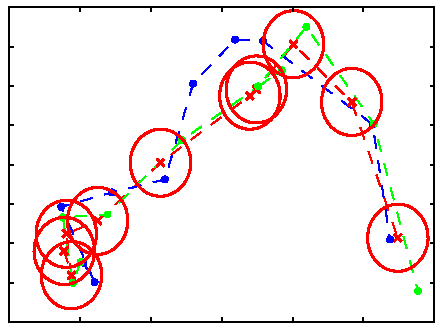
\includegraphics[width=0.5 \textwidth]{Figure13-22}
       \caption{ \label{fig:Kalman-tracking} Kalman filtering for tracking of a moving object. The blue points indicate the true positions of the object in a two-dimensional space at successive time steps, the green points denote noisy measurements of the positions, and the red crosses indicate the means of the inferred posterior distributions of the positions obtained by running the Kalman filtering equations. The covariances of the inferred positions are indicated by the red ellipses, which correspond to contours having one standard deviation. \citep[Figure 13.22]{Bishop2006}}
     \end{figure}
     
      
     \end{solution}
     
   \item Explain Equation \eqref{eq:mu-def} in non-technical terms. What happens if the variance $D_s^2$ of the observation noise goes to zero?
     
     \begin{solution}
       We have already seen that $A_s \mu_{s-1}$ is the predictive
       mean of $h_s$ given $v_{1:s-1}$. The term $C_s A_s \mu_{s-1}$
       is thus the predictive mean of $v_s$ given the observations so
       far, $v_{1:s-1}$. The difference $v_s - C_s A_s \mu_{s-1}$ is
       thus the prediction error of the observable. Since $\alpha(h_s)$ is
       proportional to $p(h_s | v_{1:s})$ and $\mu_s$ its mean, we
       thus see that the posterior mean of $h_s | v_{1:s}$ equals the
       posterior mean of $h_s | v_{1:s-1}$, $A_s \mu_{s-1}$, updated
       by the prediction error of the observable weighted by the
       Kalman gain.

       For $D_s^2 \to 0$, $K_s \to C_s^{-1}$ and
        \begin{align}
          \mu_s & = A_s \mu_{s-1} + K_s \left(v_s - C_s A_s \mu_{s-1}\right) \\
          & = A_s \mu_{s-1} + C_s^{-1} \left(v_s - C_s A_s \mu_{s-1}\right) \\
          & = A_s \mu_{s-1} + C_s^{-1} v_s - A_s \mu_{s-1}\\
          & =  C_s^{-1} v_s,
        \end{align}
        so that the posterior mean of $p(h_s | v_{1:s})$ is obtained
        by inverting the observation equation. Moreover, the variance
        $\sigma_s^2$ of $h_s | v_{1:s}$ goes to zero so that the value
        of $h_s$ is known precisely and equals $C_s^{-1} v_s$.
       
     \end{solution}
\end{exenumerate}

